\section*{Schaltungssimulation in Octave, Aufgabe 2.3}\label{sec:ag2.3}
\addcontentsline{toc}{section}{Schaltungssimulation in Octave, Aufgabe 2.3}
Eine numerische Simulation von linearen Schaltungen kann auch in Octave vor genommen werden. Hierzu wurden bereits die beiden Methoden \texttt{prs\_spice} (Methode zum Auslesen der Netzliste) und \texttt{dassl} (Methode zum nummerischen Lösen von Differenzialgleichungen) bereit gestellt.
Die Aufgabe wurde nun in 3 einzelne Skripte unterteilt:

\subsection*{Methode \texttt{circuit\_matrices}}
	Methode \texttt{circuit\_matrices} (siehe \ref{circuit_matrices}) berechnet alle Matrizen, die für die modifizierte Knotenanalyse benötigt werden. Rückgabewerte sind die Matrizen $\mathbf{A_C, A_L, A_R, A_V, A_I, C, L, G}$ sowie die Vektoren $\mathbf{v}$ und $\mathbf{i}$. Hierbei stellen die Variablen $\mathbf{A}$ so genannte Inzidenzmatrizen dar, also Matrizen, die Auskunft über die Beziehungen der Knoten und Kanten eines Graphen geben. In diesem Fall wird für jeden Typ Bauteil (Kondensator $C$, Spule $L$, Widerstand $R$, Spannungsquelle $V$ und Stromquelle $I$) eine Matrix erstellt, deren Einträge folgender Eigenschaft genügen:
	\begin{equation}
	a_{ij} = \begin{cases}
	+1 & \text{falls Zweig }j \text{ mit Bauteil von Knoten }i \text{ weg führt} \\
	-1 & \text{falls Zweig }j \text{ mit Bauteil zu Knoten }i \text{ hin führt} \\
	0  & \text{sonst}
	\end{cases}
	\end{equation}
	$\mathbf{C, L}$ und $\mathbf{G}$ stellen Diagonalmatrizen dar, die die Zahlenwerte der Bauteile enthalten (Induktivitäten in
	Henry, Kapazitäten in Farad, Leitfähigkeiten in Siemens). Zuletzt gibt die Methode die Vektoren $\mathbf{v}$ und $\mathbf{i}$ zurück, welche konstante Ströme oder Spannungen der Quellen enthalten.
	
\subsection*{Methode \texttt{calculate\_matrices}}
	Methode \texttt{calculate\_matrices} (siehe \ref{calculate_matrices}) setzt die zuvor berechneten Matrizen zu größeren Matrizen zusammen, die die Differenzialgleichung
	\begin{equation}
	\mathbf{M} \frac{\text{d}}{\text{d}t} \mathbf{x} + \mathbf{K} \mathbf{x} = \mathbf{r}
	\label{eq:matrixDGL}
	\end{equation}
	beschreiben. Rückgabewerte sind die Matrizen $\mathbf{M, K}$ und der Spaltenvektor $\mathbf{r}$, die sich nach folgender Rechenvorschrift ergeben:
	\begin{equation}
	\underbrace{
		\begin{bmatrix}
			\mathbf{A_C C A_C^T} & \mathbf{0} & \mathbf{0}\\
			\mathbf{0} & \mathbf{L} & \mathbf{0}\\
			\mathbf{0} & \mathbf{0} & \mathbf{0}
		\end{bmatrix}
	}_{\coloneqq \mathbf{M}}
	\frac{\text{d}}{\text{d}t}
	\begin{bmatrix}
		\boldsymbol{\varphi}\\
		\mathbf{i_L}\\
		\mathbf{i_L}
	\end{bmatrix}
	+
	\underbrace{
		\begin{bmatrix}
		\mathbf{A_R G A_R^T} & \mathbf{A_L} & \mathbf{A_V}\\
		-\mathbf{A_L^T} & \mathbf{L} & \mathbf{0}\\
		-\mathbf{A_V^T} & \mathbf{0} & \mathbf{0}
		\end{bmatrix}
	}_{\coloneqq \mathbf{K}}
	\begin{bmatrix}
	\boldsymbol{\varphi}\\
	\mathbf{i_L}\\
	\mathbf{i_L}
	\end{bmatrix}
	=
	\underbrace{
		\begin{bmatrix}
			-\mathbf{A_I i_S}\\
			\mathbf{0}\\
			-\mathbf{v_S}
		\end{bmatrix}
	}_{\coloneqq \mathbf{r}}
	\end{equation}
	\newpage

\subsection*{Finales Skript}	
	Das finale Skript (siehe \ref{finalesSkript}) löst nun die in \ref{eq:matrixDGL} beschriebene Differenzialgleichung auf nummerischen Weg. Dazu wird eine bereits in Octave implementierte Methode namens \texttt{dassl} verwendet. Diese bekommt den Term der Form $\mathbf{M} \frac{\text{d}}{\text{d}t} \mathbf{x} + \mathbf{K} \mathbf{x} - \mathbf{r}$ übergeben. Ebenso benötigt die Funktion die Anfangswerte $\mathbf{x_0}$ und $\mathbf{\dot{x}_0}$ sowie einen Vektor $\mathbf{t}$ mit Zeitpunkten, für die die Lösung berechnet werden sollen.

	Durch nummerische Annäherungsverfahren bestimmt die Methode den gesuchten Vektor $\mathbf{x}$ zum Zeitpunkt $t$. Dieser Lösungsvektor $\mathbf{x}$ enthält in diesem Fall die Werte
	\begin{equation}
	\mathbf{x} =
	\begin{bmatrix}
		\varphi_1\\
		\varphi_2\\
		i_L
	\end{bmatrix},
	\end{equation}
	also die beiden Potenziale $\varphi_1, \varphi_2$ an Knoten 1 und 2, sowie den Strom durch die Spule $i_L$ (siehe \ref{schaltplan}).
	Durch einzeichnen der verschiedenen Lösungen mithilfe der Methode \texttt{plot}, lässt sich der zeitliche Verlauf des Systems betrachten:
	
	\begin{figure}[h]
		\centering
		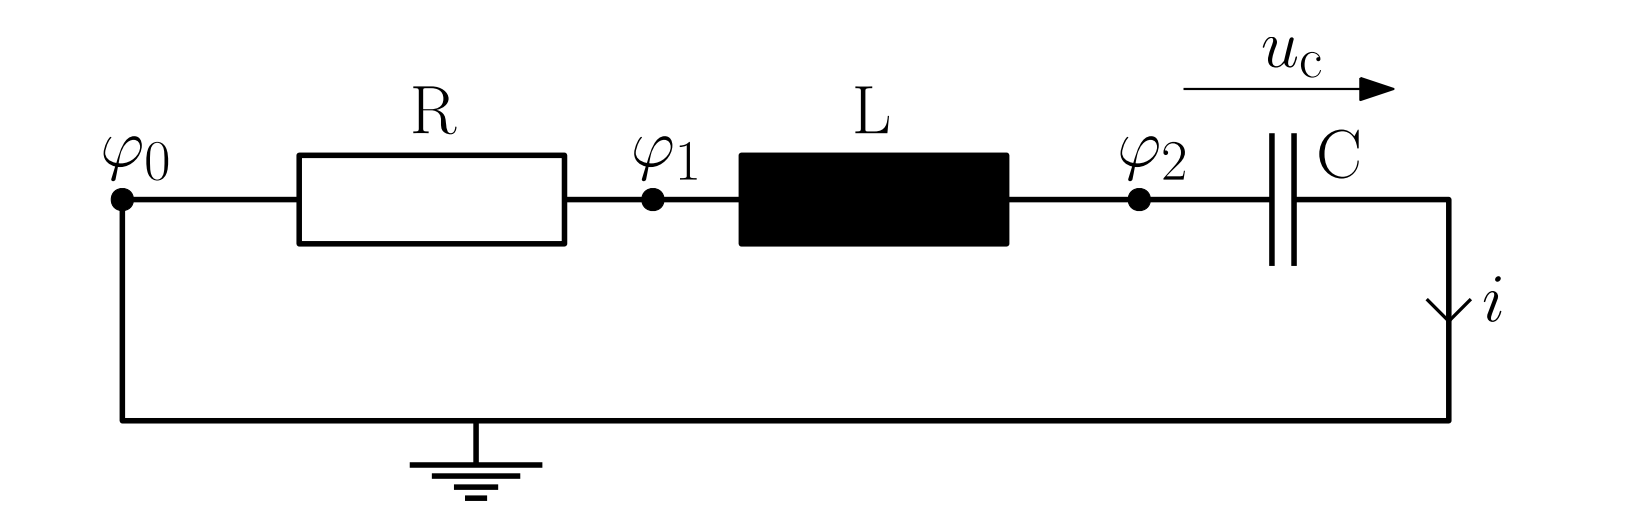
\includegraphics[width=0.65\textwidth]{data/schaltplan}
		\caption{\centering Schaltplan des harmonischen Oszillators mit $R=2\si{\ohm}$, $L=1.73007\si{\milli\henry}$ und $C=10\si{\micro\farad}$}
		\label{schaltplan}
	\end{figure}
	
	\begin{figure}[t]
		\centering
		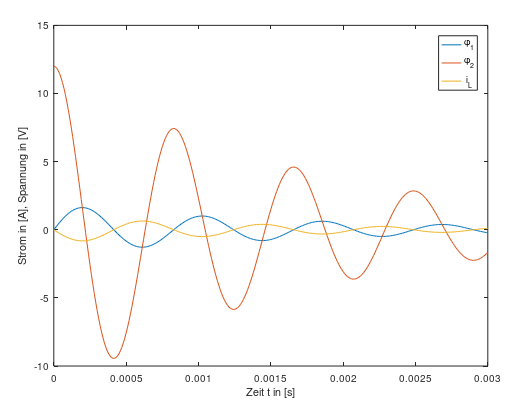
\includegraphics[width=0.76\textwidth]{data/plot}
		\caption{Schaltungssimulation des harmonischen Oszillators in \ref{schaltplan}. Initialisiert mit Anfangsspannung $u_C = 12V$ am Kondensator zum Zeitpunkt $t = 0$ }
		\label{plot}
	\end{figure}
\newpage
Hierbei entspricht $\varphi_1 = -u_R$ (der negativen Spannung am Widerstand), $\varphi_2 = u_C$ (der Spannung am Kondensator) und $i_L = i$ (Identisch zum Gesamtstrom, da es nur einen Strom im System gibt).

Hinweis zu den in \ref{finalesSkript} berechneten Anfangswerten $\mathbf{x_0}$ und $\mathbf{\dot{x}_0}$:

Diese müssten theoretisch per Hand für jede neue Schaltung und Art der Initialisierung des Systems neu berechnet werden. Jedoch scheinen auch inkorrekte Anfangswerte zum selben Ergebnis zu führen, was uns daraus schließen ließ, dass das numerische Annäherungsverfahren der \texttt{dassl}-Funktion, auch bei teilweise falschen Anfangswerten, zum richtigen Ergebnis konvergieren kann.
